\section{Information about some entity(s)}
\label{sec-information-about}

\textbf{Created by:} Arkopaul Sarkar \\
\textbf{Modified by:}

\subsection*{Scenario Objective}
This scenario illustrates how various types of information about an entity (e.g., object, process, properties) can be captured. This scenario introduces the fundamental classes and properties to model information. Although IOF contains many types of informational entities, this scenario only introduces the generic types of information based on how they refer to the entities they are about.  

\subsection*{General Pattern Description}

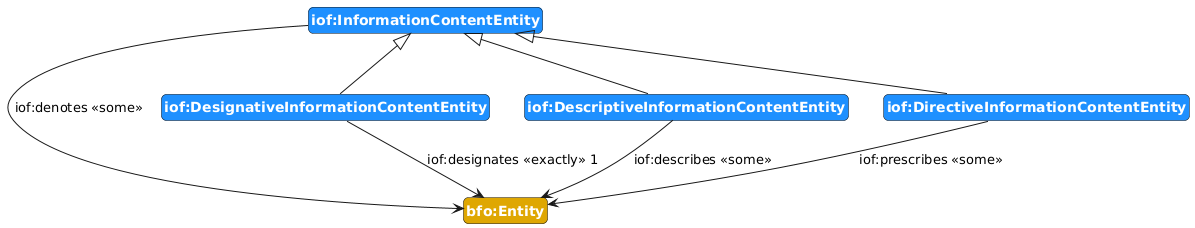
\includegraphics[scale=0.35]{scenarios/information-and-aboutness/images/general-information-aboutness.png}

The primitive and generic relationship \texttt{iof:isAbout} establishes a connection between an Information Content Entity (ICE) and a referenced entity, encapsulating the fundamental notion of ``aboutness''—that is, the ICE instance conveys information about the entity.

Three distinct modes of referring to an entity are captured through three specialized sub-properties of \texttt{iof:isAbout}: \texttt{iof:denotes} serves to distinguish one or more instances of an entity.
\texttt{iof:designates}, a functional specialization of \texttt{iof:denotes}, uniquely identifies a single specific instance, ensuring exclusive reference.
\texttt{iof:describes} conveys attributes or characteristics of an entity without necessarily providing unique identification. It emphasizes detailing the entity rather than establishing a direct referential link.
\texttt{iof:prescribes} refers to entities that may not yet exist but are expected to adhere to prescribed rules, guidelines, or specifications once instantiated. It thus encompasses potential future entities, such as artefacts constructed according to a design specification or processes executed in alignment with a plan specification.
Accordingly, the IOF Core ontology defines three corresponding classes of ICE—Designative ICE, Descriptive ICE, and Prescriptive ICE — each qualified based on these three sub-properties of \texttt{iof:isAbout}. 

\subsection*{Use Case: Information about a car}
In this use case, information about a car are asserted using different types of ``about-ness'' relations. The types of the ICE instances may be inferred based on the asserted sub-property of \texttt{iof:isAbout}. In this example, the VIN of the car acts as a unique identifier of the vehicle and the model of the car denotes the structural style of the car. A branding slogan euphemistically describes the car's ability. Lastly, a directive from the Department of Transportation prescribes the car's weight rating, i.e., the car follows the specifications for a passenger car as prescribed by `Gross Vehicle Weight Rating (GVWR)' from the Department of Transportation.   

\subsubsection*{Use Case Pattern Description}

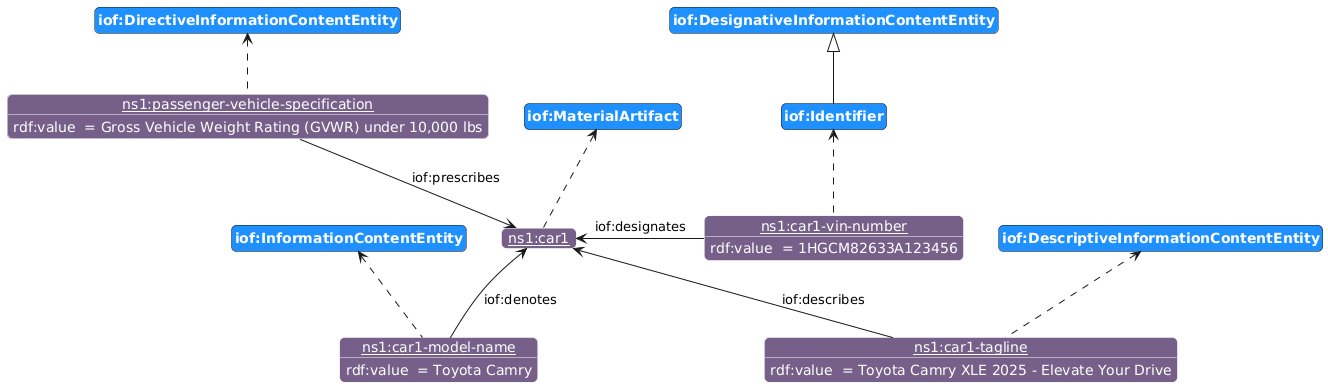
\includegraphics[scale=0.35]{scenarios/information-and-aboutness/images/uc1-ices.png}

The designative information content entity (iof:designates) uniquely identifies a specific instance of the car, typically using a Vehicle Identification Number (VIN) or a similar unique identifier, ensuring that a particular vehicle unit is individually referenced within a system. The denotative information content entity (iof:denotes) assigns a model name (Toyota Camry) to the vehicle, referring to a general category rather than an individual instance, which helps differentiate between different models within a brand. The descriptive information content entity (iof:describes) provides branding and marketing information, such as the tagline "Toyota Camry XLE 2025 – Elevate Your Drive", which conveys the product’s perception but does not serve as a unique identifier.

Meanwhile, the directive information content entity (iof:prescribes) applies to regulatory constraints, such as "Gross Vehicle Weight Rating (GVWR) under 10,000 lbs", ensuring compliance with passenger vehicle classification standards before the car is operational. The ontology’s structured approach enables semantic differentiation between designation (unique instance reference), denotation (model reference), description (attributes and perception), and prescription (rules and requirements). This classification ensures that different stakeholders—manufacturers, regulators, marketers, and data systems—can process and interpret vehicle-related information accurately for production, sales, legal compliance, and operational tracking.

\subsubsection*{Use-Case Example Data}

\begin{verbatim}
PREFIX iof: <http://example.org/iof#>
PREFIX rdf: <http://www.w3.org/1999/02/22-rdf-syntax-ns#>
PREFIX ns1: <http://example.org/ns1#>

INSERT DATA {
  ns1:car1 a iof:MaterialArtifact .
  ns1:car1-vin-number a iof:Identifier ;
      iof:designates ns1:car1 ;
      rdf:value "1HGCM82633A123456" . # Example VIN
  ns1:car1-model-name a iof:InformationContentEntity ;
      iof:denotes ns1:car1 ;
      rdf:value "Toyota Camry" .
  ns1:car1-tagline a iof:DescriptiveInformationContentEntity ;
      iof:describes ns1:car1 ;
      rdf:value "Toyota Camry XLE 2025 – Elevate Your Drive" .
  ns1:passenger-vehicle-specification a iof:DirectiveInformationContentEntity ;
      iof:prescribes ns1:car1 ;
      rdf:value "Gross Vehicle Weight Rating (GVWR) under 10,000 lbs" .
}    
\end{verbatim}


\subsubsection*{Data Mapping}


\subsubsection*{Data Validation}
